%Tech Science Press

%=================================================================
\documentclass[journal,article,submit,moreauthors,pdftex]{Definitions/tsp} 
\input{Definitions/package}
\include{Definitions/unicode}

%----------
% journal
%----------
% % Choose between the following TSP journals:
%biocell, chd, cju, cl, cmc, cmes, csse, dedt, ecn, ee, fdmp, fhmt, iasc, icces, ijimh, jai, jbd, jbic, jcs, jihpp, jimh, jiot, jnm, jpa, jpm, jqc, jrm, oncologie, or, phyton, rig, sdhm, zkg.
%--------------
% article type
%--------------
% The default manuscript type is article; alternative options include:
%abstract, analysis, article, biographicalitem, casereport, commentary, communication, correction, editorial, guideline, howidoiit, introduction, letter, legends, minireview, openforum, perspective, proceedings, protocol, retraction, review, shortcommunication, technicalreport, theory, tutorial, viewpoint

%---------------
% submit status
%---------------
%Upon acceptance, the Editorial Office will switch the class option from "submit" to "accept". This change applies only to the front page, headings, and copyright information, and will remove line numbering. Journal information and pagination will be assigned by the Editorial Office.

%------------------
% moreauthors
%------------------
% If there is only one author the class option oneauthor should be used. Otherwise use the class option moreauthors.

%---------
% pdftex
%---------
% The option "pdftex" should be used only with pdfLaTeX. For compilation with LaTeX + dvi2pdf (e.g., when using EPS figures) or XeLaTeX, this option must be removed.

%=================================================================
% Internal commands: Article information and pagination will be assigned by the Editorial Office
\continuouspages{}
\firstpage{1} 
\makeatletter 
\setcounter{page}{\@firstpage} 
\makeatother
\pubvolume{0}
\issuenum{0}
\elocationid{0}
\articlenumber{0}
\pubyear{2026}
\copyrightyear{2026}
\datereceived{Day Month Year}
\dateaccepted{Day Month Year}
\dateonlinefirst{}
\datepublished{Day Month Year}
%\datecorrected{} % For corrected papers: "Corrected: XXX" date in the original paper.
%\dateretracted{}  % For corrected papers: "Retracted: XXX" date in the original paper.

%=================================================================
% Please add packages and commands here. The following packages are loaded in the class file: fontenc, inputenc, calc, indentfirst, fancyhdr, graphicx, epstopdf, lastpage, ifthen, lineno, float, amsmath, setspace, enumitem, mathpazo, booktabs, titlesec, etoolbox, tabto, xcolor, soul, multirow, microtype, tikz, refcount, totcount, attrib, amsthm, upgreek, array, tabularx, pbox, ragged2e, tocloft, adjustbox, enotez, subfig
%\usepackage{combelow}
\usepackage[OT1,OT2,T2A,T2B,T2C,T3,T5,T1]{fontenc}
\usepackage[russian,english]{babel}

%=================================================================
%% Please use the following mathematics environments: Theorem, Lemma, Corollary, Proposition, Characterization, Property, Problem, Example, ExamplesandDefinitions, Hypothesis, Remark, Definition, Notation, Assumption
%% For proofs, please use the proof environment (the amsthm package is loaded by the TSP class).
%\begin{Theorem}
%\end{Theorem}
%\begin{proof}
%\end{proof}

%=================================================================
% Full title of the paper (Capitalized)
\Title{Title}
%\TitleCitation{Title} %for citaion purposes

% Author Orchid ID: enter ID or remove command
%\newcommand{\orcidauthorA}{0000-0000-000-000X} % Add \orcidA{} behind the author's name
%\newcommand{\orcidauthorB}{0000-0000-000-000X} % Add \orcidB{} behind the author's name

% Authors, for the paper (add full first names)
\Author{Firstname Lastname\textsuperscript{1}, Firstname Lastname\textsuperscript{2} and Firstname Lastname\textsuperscript{2,*}}
%\AuthorCitation{Lastname F, Lastname F, Lastname F}%for citaion purposes

% Authors, for metadata in PDF
\AuthorNames{Firstname Lastname, Firstname Lastname and Firstname Lastname}

% Affiliations / Addresses (Add [1] after \address if there is only one affiliation.)
\address{%
\textsuperscript{1}Affiliation 1 (Department/School/Faculty/Campus/\dots, University/\dots), City, Country

\textsuperscript{2}Affiliation 2, City, Country
}%

% Contact information of the corresponding author
\corres{Corresponding Author: Author’s Name. Email: author@institute.xxx}

% Current address and/or shared authorship
%\firstnote{These authors contributed equally to this work} % Optional: can be left empty if unnecessary
%The commands \thirdnote{} till \myeighthnote{} are available for further notes

%\secondnote{Current address: Affiliation} % Optional: can be left empty if unnecessary
%Current address must not duplicate any entry in the Affiliation section.

% Abstract (Do not use inserted blank lines, i.e. \\)
\abstract{Please type your abstract here. Abstracts of a research paper should be typically 200 to 400 words in length, and 150 to 300 words for a review paper. We encourage authors to use the following style of structured abstracts, but without headings, e.g., (1) Background: Outline the broader context of the research and specify the study’s objective. (2) Methods: Describe the principal methods or procedures employed. (3) Results: Summarize the major findings. (4) Conclusions: State the key conclusions or interpretations drawn from the results. Abstracts shall not include reference citations. Abbreviations that appear only once in the abstract should be defined in full. If abbreviations appear more than once, the full definitions should be provided first before they can be used elsewhere.}

% List 3 to 10  pertinent keywords specific to the article, yet reasonably common within the subject discipline.
\keyword{Keyword 1; keyword 2; keyword 3 (List 3 to 10 pertinent keywords specific to the article yet reasonably common within the subject discipline)}  

%  PACS, MSC, and JEL can be left empty or commented out if not applicable
%\PACS{}
%\MSC{}
%\JEL{}

%%%%%%%%%%%%%%%%%%%%%%%%%%%%%%%%%%%%%%%%%%%
\begin{document}

\section{Introduction} \label{sect:s1}
In introduction, authors should provide a context or background for the study (the nature of the problem and its significance). State the specific purpose or research objective of, or hypothesis tested by, the study or observation. Cite only directly pertinent references, and do not include data or conclusions from the work being reported.
 

\section{Structure} \label{sect:s2}
A manuscript should include the following sections: Title, Author Names with Affiliations, Abstract, Keywords, Main Text (for Articles, a structured format, e.g., Introduction, Results, Discussion, Methods, Conclusions, is recommended, while Reviews may use a more flexible structure), Acknowledgement, Funding Statement, Author Contributions, Availability of Data and Materials, Ethics Approval, Conflicts of Interest, Supplementary Materials (if any), Glossary (if any), Appendix (if any), and References.

\subsection{Text Layout} \label{sect:s2dot1}
Paper size: US Letter (8.5″ $\times$ 11″ or 21.59 cm $\times$ 27.94 cm).

Paper Layout: Single column, Single spaced.

Use 0.75 cm indent on the first line of each new paragraph. Use single line spacing, 3 pt spacing after the paragraph. All levels of headings should use 12 pt spacing before, 3 pt after.

\subsection{Headings} \label{sect:s2dot2}
Please capitalize all initial letters of substantives of headings.
\begin{enumerate}[label=$\bullet$]
\item Level 1 headings for sections should be in bold, 11 pt, and be flushed to the left. Level 1 heading should be numbered using Arabic numbers, such as 1, 2, 3, \dots
\item Level 2 headings for subsections should be in bold-italic, 11 pt, and be flushed to the left. Level 2 headings should be numbered after the level one heading. For example, the second level two heading under the third level one heading should be numbered as 3.2.
\item Level 3 headings should be in italic, 11 pt, and be flushed to the left. Similarly, the level 3 headings should be numbered after the level two headings, such as 3.2.1, 3.2.2, \dots
\item Level 4 headings should be in not italic and not bold, 11 pt, and be flushed to the left. Level 4 headings should not be numbered. This is the last level of headings permitted.
\end{enumerate}


\section{Figures and Tables} \label{sect:s3}
Figures and Tables must be numbered consecutively using Arabic numerals and placed within the text immediately following their first citation to maintain a seamless flow and clarity in the presentation. The first citation of figures and tables in the main text must follow a sequential order.

\subsection{Figures} \label{sect:s3dot1}
Figures should be centered and should have a figure caption placed underneath. Figures should have clear and relevant legends, without duplicating information already presented in the main text.

\subsubsection{Figure Body} \label{sect:s3dot1dot1}
\begin{enumerate}[label=$\bullet$]
\item Figures should be scaled to fit within the allowable space while preserving their original proportions and avoiding distortion. The preferred format is .tif, with RGB color space, a DPI of 500+ (accepted image resolutions: Line Art $\geq$ 900 dpi, Halftone $\geq$ 300 dpi, Combo $\geq$ 600 dpi), no alpha channels, and flattened layers;
\item Images must be clear and complete, with no obscured text or content. Scale bars and numerical labels should be legible, and images should be free of watermarks;
\item Unnecessary marks such as red wavy lines and hard (soft) returns are not allowed in figures;
\item To avoid any errors during position changes, please provide the combined image instead of editable pieces in figures;
\item Any special characters or icons in an image (e.g., *, **, ***, \textsuperscript{abc}, \textsuperscript{123}$\dots$) need to have a corresponding explanation (can be added in the image or caption);
\item Sub-figure labels must be clear, proportional, consistently formatted in standard fonts (e.g., Arial, Helvetica), sized between 8--11 point, in black, and free from overlap, distortion, or formatting errors;
\item Duplicate images or repeated figure numbers are not allowed;
\item References in the form of “[xx]” are not recommended in the image. If necessary, “Author + Year” format can be used in the image, and all mentioned references must be cited in the caption.
\end{enumerate}

\subsubsection{Figure Captions} \label{sect:s3dot1dot2}
One-line captions should be centered in the column. Refer to \fig{fig:fig-1} below as an example:
\begin{figure}[H]
\centering

\includegraphics[scale=1]{Definitions/image-f001.pdf}
\caption{This is a figure example. Please remove all non-English terms or add a definition for them.}
\label{fig:fig-1}
\end{figure}   

Multi-line captions should be justified on both sides. Refer to \fig{fig:fig-2} below as an example:

\begin{figure}[H]
\centering
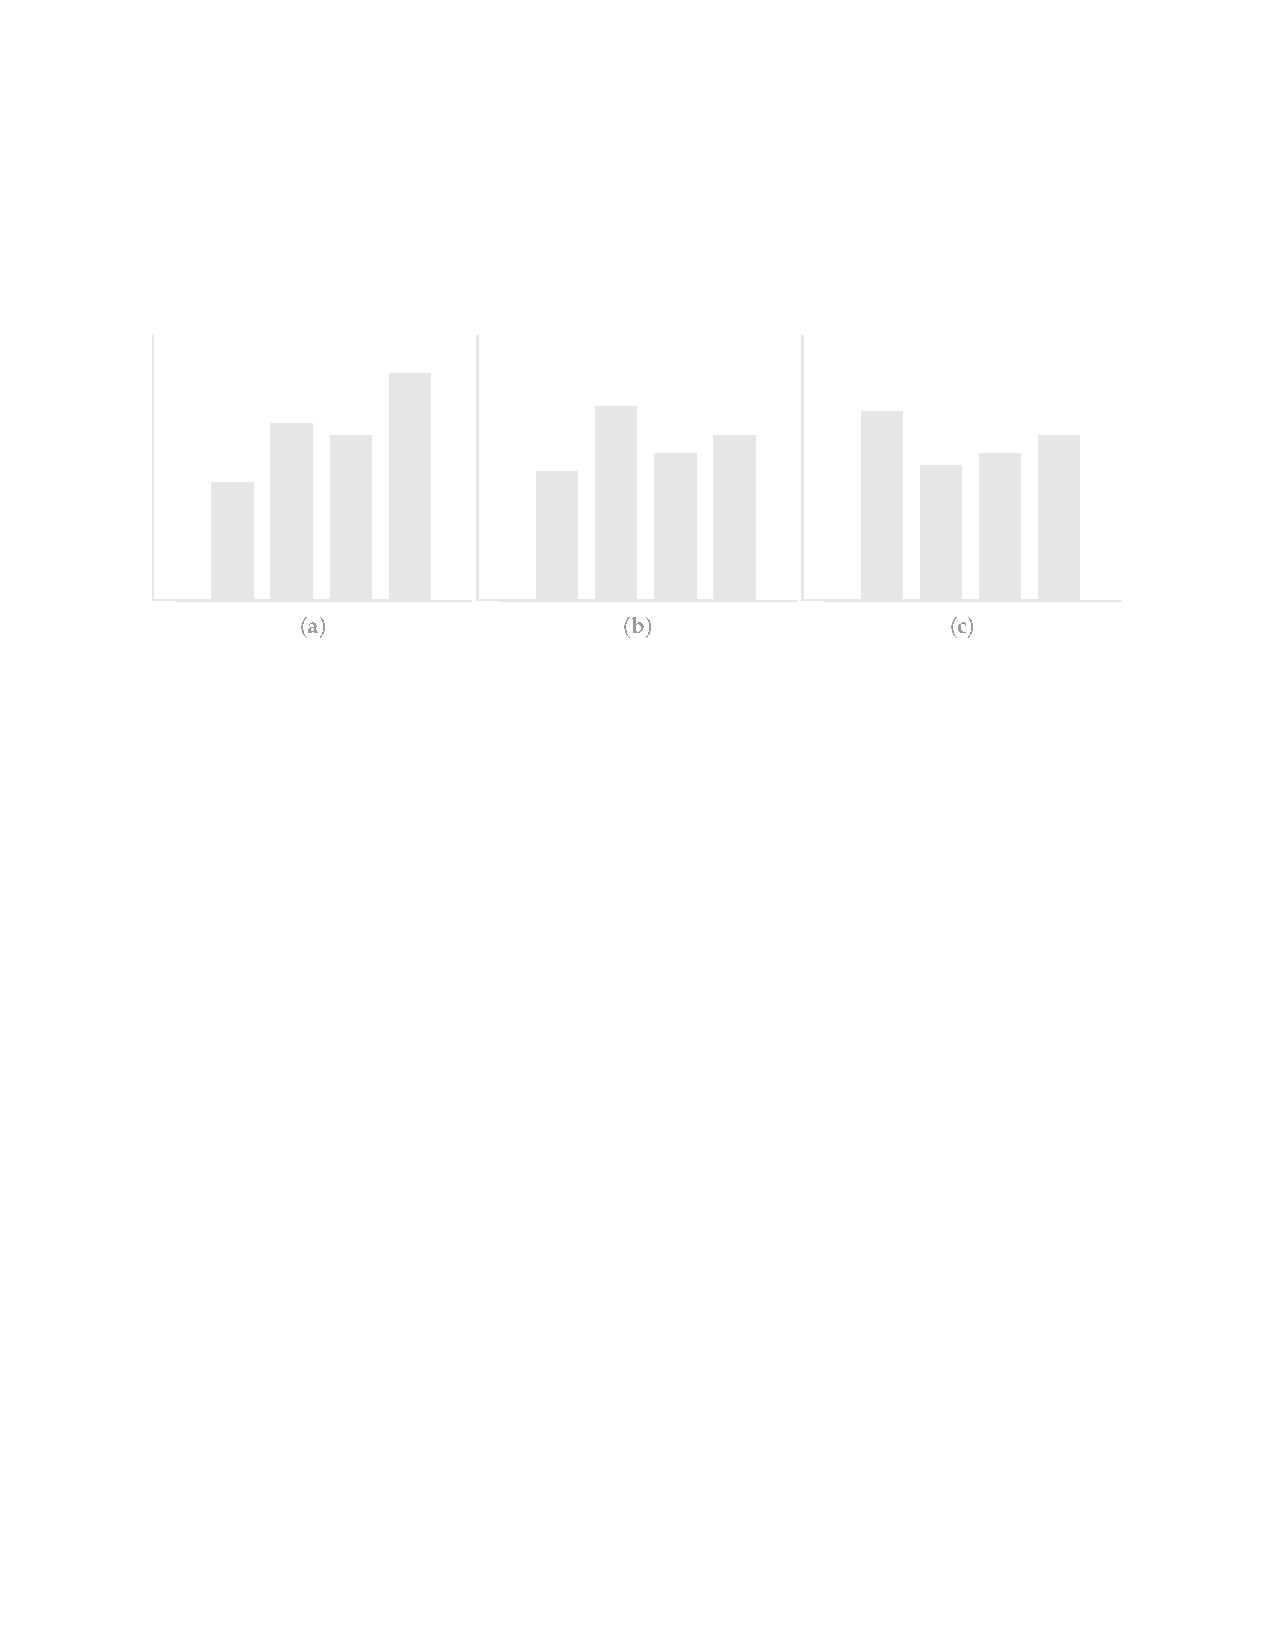
\includegraphics[scale=1]{Definitions/image-f002.pdf}
\caption{This is an example of a figure with sub-figures. All special symbols and markers in the image require corresponding explanations in the caption. If there are multiple panels, they should be listed as: (\textbf{a}) Description of what is contained in the first panel; (\textbf{b}) Description of what is contained in the second panel; (\textbf{c}) Description of what is contained in the third panel. Ensure that permission has been obtained and there is no copyright issue. If copyright is needed, please provide a citation in the following format: “Reprinted/adapted with permission from reference [xx]. Copyright year, copyright owner’s name.”}
\label{fig:fig-2}
\end{figure}   

When citing multiple figures, use the following formats: \cref{fig:fig-1,fig:fig-2}, Figs. 1--3, Fig. 2a,b, Fig.~2a--c. 
%\cref{fig:fig-1,fig:fig-2}, \cref{fig:fig-1,fig:fig-2,fig:fig-3}, \fig{fig:fig-2}a,b, \fig{fig:fig-2}a--c

\subsection{Tables} \label{sect:s3dot2}
\subsubsection{Table Body} \label{sect:s3dot2dot1}
\begin{enumerate}[label=$\bullet$]
\item Tables should be centered, should not be wrapped by text, and should have captions placed above;
\item All tables must be submitted in an editable format and not as embedded images;
\item Sub-tables, e.g., Table 1a and Table 1b, must be either merged into a single table or split into separate individual tables;
\item Font color, background color, italics, bold, underlines, etc., in tables must be clearly explained; otherwise, they should be removed;
\item Any special characters or icons in a table (e.g., *, **, ***, \textsuperscript{abc}, \textsuperscript{123}$\dots$) need to have a corresponding explanation (in table footers or captions).
\end{enumerate}

\subsubsection{Table Captions \& Footer} \label{sect:s3dot2dot2}
Table captions should be centered (See \tabref{tabref:table-1}). If the caption has more than one line, the text should be aligned justified on both ends.

\begin{table}[H] 
\tablesize{\footnotesize}
\caption{This is a table caption. Please add an explanation for bold/italics/underline/color to the table footer.}
\label{tabref:table-1}
\newcolumntype{C}{>{\centering\arraybackslash}X}
\begin{tabularx}{\textwidth}{CCCC}
\toprule
\textbf{Header 1} & \textbf{Header 2} & \textbf{Header 3} & \textbf{Header 4}\\
\midrule
data* & data & data & data\\
data & data & data & data\textsuperscript{1}\\
\bottomrule
\end{tabularx}
\footnotesize{This is a table footer. *The special symbols should be explained in the table footer; \textsuperscript{1}The special markers should be explained in the table footer. Ensure that permission has been obtained and there is no copyright issue. If copyright is needed, please provide a citation in the following format: “Reprinted/adapted with permission from Reference [xx]. Copyright year, copyright owner’s~name.”}
\end{table}

When citing multiple tables, use the following formats: Tables 1 and 2, Tables 1--3, Tables 1, 2 and 4.
%\cref{tabref:table-1,tabref:table-2}, \cref{tabref:table-1,tabref:table-2,tabref:table-3}, \cref{tabref:table-1,tabref:table-2,tabref:table-4}


\section{Equations and Mathematical Expressions} \label{sect:s4}
Equations and mathematical expressions must be inserted into the main text.  Formulas must not be inserted as images. Authors may format formulas in either in-line or display style.

\subsection{In-Line Style}\label{sect:s4dot1}
In-line equations/expressions are embedded into the paragraphs of the text. For example,  $E = mc^2$. In-line equations or expressions should not be numbered.

\subsection{Display Style}\label{sect:s4dot2}
Equations in display format should be separated from the surrounding text, aligned to the left of the column, with the equation label aligned to the right margin. Equations should be editable and numbered consecutively in Arabic numerals within parentheses, where applicable. See Eq. (1) for an example:
\begin{equation}
E = mc^2
\tag{1}
\end{equation}
the text following an equation need not be a new paragraph. Please punctuate equations as regular text. When citing multiple equations, please use the format: Eqs. (1) and (2), Eqs. (1)--(3),  Eqs. (1), (2) and (4).

\subsection{Mathematical Expressions}\label{sect:s4dot3}
Theorem-type environments (including propositions, lemmas, corollaries, etc.) can be formatted as~follows:
\begin{Theorem}
Example text of a theorem (Text should be italic). Theorems, propositions, lemmas, etc., should be numbered sequentially (i.e., Theorem 2 follows Theorem 1). 
 
Examples or Remarks use the same formatting, but should be numbered separately, so a document may contain Theorem 1, Remark 1 and Example 1.
\end{Theorem}

The text continues here. Proofs must be formatted as follows:

\begin{proof}[Proof of Theorem 1]
 Text of the proof. Note that the phrase “of Theorem 1” is optional if it is clear which theorem is being referred to. Always finish a proof with the following symbol.
\end{proof}

The text continues here.


\section{Statements} \label{sect:s5}
\textls[-10]{Please note that the 6 pieces of information (Acknowledgement, Funding Statement, Author Contributions, Availability of Data and Materials, Ethics Approval, Conflicts of Interest) need to be truthfully provided at the end of the article.}

\acknowledgement{This section is intended for acknowledging any support not covered under the Author Contributions or Funding Statement sections. This may include administrative and technical assistance, as well as in-kind contributions such as materials or equipment provided for the research. Please be aware that the specific funding grant number should only appear in the Funding Statement. If there are no acknowledgement to be made, please use “Not applicable.” or “None.”}

\funding{Authors should describe sources of funding that have supported the work, including specific grant numbers, initials of authors who received the grant, and the URLs to sponsors’ websites: “This research was funded by Name of Funder, grant number xxx.” or “The APC was funded by xxx.” Please ensure that all funding information is accurate and that the names of funding agencies are spelled according to the standard forms listed at \href{https://search.crossref.org/funding}{https://search.crossref.org/funding}. Inaccuracies may affect the traceability of your work and future funding recognition. If there is no funding support, please write “The author(s) received no specific funding for this study.”}

\authorcontributions{The Author Contributions statement is mandatory for research articles, except for papers with a single author. It should represent all the authors and is to be included upon submission. All listed authors must have substantially contributed to the manuscript and have approved the final submitted version, which should include a description of each author’s specific work and contribution. We suggest the following format for the contribution statement:\\
“The authors confirm contribution to the paper as follows: Conceptualization, First-name Lastname1 and First-name Lastname2; methodology, First-name Lastname1; software, First-name Lastname1; validation, First-name Lastname1, First-name Lastname2 and First-name Lastname3; formal analysis, First-name Lastname1; investigation, First-name Lastname1; resources, First-name Lastname1; data curation, First-name Lastname1; writing---original draft preparation, First-name Lastname1; writing---review and editing, First-name Lastname1; visualization, First-name Lastname1; supervision, First-name Lastname1; project administration, First-name Lastname1; funding acquisition, First-name Lastname1. All authors reviewed and approved the final version of the manuscript.”\\
Please turn to the \href{https://credit.niso.org/contributor-roles-defined/}{CRediT role descriptors---CRediT} for the term explanation.}

\availabilityofdataandmaterials{This statement should make clear how readers can access the data used in the study and explain why any unavailable data cannot be released. The following five statements are offered for~reference:
\begin{enumerate}
\item Data openly available in a public repository.
\item[] “The data that support the findings of this study are openly available in [repository name] at [URL].”
\item Data available within the article or its Supplementary Materials.
\item[] “The authors confirm that the data supporting the findings of this study are available within the article [and/or] its Supplementary Materials.”
\item Data available on request from the authors.
\item[] “The data that support the findings of this study are available from the Corresponding Author, [author initials], upon reasonable request.”
\item Data not available due to [ethical/legal/commercial] restrictions.
\item[] “Due to the nature of this research, participants of this study did not agree for their data to be shared publicly, so supporting data is not available.”
\item “Not applicable.” (This article does not involve data availability, and this section is not applicable).
\end{enumerate}}

\ethicsapproval{Guidelines for ethical approval statements may differ based on the journal, a standard ethical approval statement will usually include:
\begin{enumerate}
\item Whether or not the study included human or animal subjects. In all cases, the ethical approval status of the work should be stated in the ethical approval statement.
\item The committee which approved the study.
\item The compliance documents. What policies, declarations, acts, etc.
\item Persistent identifier: reference or approval number. Include the registration ID/reference number if applicable.
\item “Not applicable.” for studies not involving humans or animals.
\end{enumerate}}

\conflictsofinterest{Please declare conflicts of interest or state: “The authors declare no conflicts of interest.” Authors must disclose any personal interests that could bias the research. Any role of funders in study design, data collection, analysis, manuscript preparation, or publication decisions must be stated. If funders had no involvement, please include the statement: “The funders had no role in the design of the study; in the collection, analyses, or interpretation of data; in the writing of the manuscript; or in the decision to publish the results.”} 

%% Optional
\supplementary{The supplementary material is available online at \linksupplementary{}, Figure S1: caption; Table S1: caption; Video S1: caption.\\
Supplementary Materials should be uploaded separately on submission.  Any file format is acceptable; however, we recommend that common, non-proprietary formats are used where possible. Supplementary materials should be clean, without tracked changes, highlights, comments or line numbers. Supplementary figures must be clear and readable, and we recommend a minimum resolution of 300 dpi, figure legends must be clear and accurate. Supplementary materials must be mentioned in the main text. The citation format of Supplementary Figures, Tables, Equations, etc., should start with a prefix “S”, e.g., Fig. S1, Table S1, Eq. (S1), etc.}


%% Optional
\abbreviations{Abbreviations}{\indent The following abbreviations are used in this manuscript:\\

\noindent 
\begin{tabular}{@{}ll}
Term 1 & Interpretation 1\\
Term 2 & Interpretation 2\\
Term 3 & Interpretation 3
\end{tabular}}

%% Optional
\appendixstart
\appendix
\section[\appendixname~\thesection]{ } \label{app:app1}
\subsection[\appendixname~\thesubsection]{ } \label{app:app1dot1}
The appendix is an optional section that may include details and data supplemental to the main text---such as experimental details that would otherwise disrupt the narrative flow but are crucial to understanding and reproducibility. Mathematical proofs of results not central to the paper can be added as an appendix; brief figures showing replicate data for experiments presented in representative form in the main text may also be included in the appendix.~More extensive data should be provided as Supplementary~Materials.

\section[\appendixname~\thesection]{Example of Section Title} \label{app:app2}
Multiple appendices should be ordered as such: Appendix A, Appendix B, Appendix C, etc. Appendix sections must be cited in the main text. Within the appendices, figures, tables, and other elements should be labeled starting with “A”, derived from the initial letter of “Appendix”---e.g., Figure A1, Figure A2, \tabref{tabref:table-a1}, Algorithm A1, etc.

\begin{table}[H] 
\tablesize{\footnotesize}
\caption{This is a table caption. Please add an explanation for bold/italics/underline/color to the table footer.}
\label{tabref:table-a1}
\newcolumntype{C}{>{\centering\arraybackslash}X}
\begin{tabularx}{\textwidth}{CCCC}
\toprule
\textbf{Header 1}	&\textbf{Header 2}	&\textbf{Header 3}	&\textbf{Header 4}\\
\midrule
data	&data	&data	&data\\
data	&data	&data	&data\\
\bottomrule
\end{tabularx}
\end{table}


%%References instruction
% Please provide either the correct journal abbreviation (e.g. according to the “List of Title Word Abbreviations” http://www.issn.org/services/online-services/access-to-the-ltwa/) or the full name of the journal.

% Citations and References in Supplementary files are permitted provided that they also appear in the reference list here. 

% All references should be cited in the main text sequentially (including citations in tables and legends) and listed individually at the end of the manuscript. We recommend preparing the references with a bibliography software package, such as EndNote, Mendeley or Zotero, to avoid typing mistakes and duplicated references. Include the digital object identifier (DOI) for all references where available.

%Citations should be generated using LaTeX citation commands (e.g., \cite{ref-1}, \cite{ref-2,ref-3}, or \cite{ref-4,ref-5,ref-6}. For citations with specific page numbers, place the page information outside the citation brackets, for example \cite{ref-5} (p.~10) or \cite{ref-6} (pp.~101--105). When a cited reference is the subject of a sentence, use the author’s last name followed by the citation command, e.g., Rhee \cite{ref-1}, or use a generic form such as Ref.~\cite{ref-1} or Refs.~\cite{ref-4,ref-5,ref-6}; for references with multiple authors, use the first author’s last name followed by “et al.”, e.g., Al-Khshali et al.~\cite{ref-2}. It is not recommended to cite more than 5 consecutive references at a single location. Citations and references in the Supplementary Materials are permitted provided that they also appear in the main reference list.

%Please include the first 6 authors’ names before using “et al.” in the references lsit.

%The following are examples of the reference style (Vancouver style), which should be strictly adhered to (More details of style can refer to: https://www.ncbi.nlm.nih.gov/books/NBK7256/).

%=====================================
% References, variant A: external bibliography
%=====================================
%\bibliography{your_external_BibTeX_file}

%=====================================
% References, variant B: internal bibliography
%=====================================

\reftitle{References}
\begin{thebibliography}{999}
%%Journal
%Author AA, Author BB. Title of article. Abbreviated Journal Name. Year;volume(issue):pagination.
%Author AA Jr, Author BB 2nd, Author CC, Author DD, Author EE, Author FF, et al. Title of article. Abbreviated Journal Name. Year;volume(issue):pagination.
\bibitem{ref-1}
Rhee HS. Chosen-ciphertext attack secure public-key encryption with keyword search. Comput Mater Contin. 2022;73(1):69--85. [\href{https://doi.org/10.32604/cmc.2022.026751}{CrossRef}]
\bibitem{ref-2}
Al-Khshali HH, Ilyas M. Impact of portable executable header features on malware detection accuracy. Comput Mater Contin. 2023;74(1):153--78. [\href{https://doi.org/10.32604/cmc.2023.032182}{CrossRef}]
\bibitem{ref-3}
Khan MA, Usman M, Zhao Y. First principles calculations for corrosion in Mg-Li-Al alloys with focus on corrosion resistance: A comprehensive review. Comput Mater Contin. 2024;81(2):1905--52. [\href{https://doi.org/10.32604/cmc.2024.054691}{CrossRef}]
\bibitem{ref-4}
Dong Y, Zhao K, Gao L, Li H. A hybrid level set optimization design method of functionally graded cellular structures considering connectivity. Comput Mater Contin. 2024;79(1):1--18. [\href{https://doi.org/10.32604/cmc.2024.048870}{CrossRef}]
\bibitem{ref-5}
Long Y, Zhong J, Zhang T, Chen L, Zhang L. Multiscale simulation of microstructure evolution during preparation and service processes of physical vapor deposited c-TiALN coatings. Comput Mater Contin. 2024;79(3):3435--53. [\href{https://doi.org/10.32604/cmc.2024.0516290}{CrossRef}]
\bibitem{ref-6}
Shoeibi M, Nevisi MMS, Salehi R, Martín D, Halimi Z, Baniasadi S. Enhancing hyper-spectral image classification with reinforcement learning and advanced multi-objective binary grey wolf optimization. Comput Mater Contin. 2024;79(3):3469--93. [\href{https://doi.org/10.32604/cmc.2024.049847}{CrossRef}]
\bibitem{ref-7}
Hong Y, Fang S, Su J, Xu W, Wei Y, Wu J, et al. A novel approach for image encryption with chaos-RNA. Comput Mater Contin. 2023;77(1):139--60. [\href{https://doi.org/10.32604/cmc.2023.043424}{CrossRef}]

%%Book
%Author AA, Author BB. Title of the book. Publisher Location: Publisher; Year. Pagination (Optional).
%Editor AA, Editor BB, editors. Title of the book. Publisher Location: Publisher; Year. Pagination (Optional).
%Author AA, Author BB. Title of the book. xth ed. (if not first) Vol. x (if any). Publisher Location: Publisher; Year. Pagination (Optional).
%Author AA, Author BB. Title of the book. xth ed. Translator AA, translator. Publisher Location: Publisher; Year. Pagination (Optional).
%Author AA, Author BB. Title of the book. Publisher Location: Publisher; Year. Section/Table/Charts/… x; Pagination (Required).
%Author AA, Author BB. Title of the chapter. In: Editor AA, Editor BB, editors. Title of the book. xth ed. (if not first) Publisher Location: Publisher; Year. Pagination (Required).
\bibitem{ref-8}
Jenkins PF. Making sense of the chest X-ray: A hands-on guide. New York, NY, USA: Oxford University Press; 2005. 194 p.
\bibitem{ref-9}
Eyre HJ, Lange DP, Morris LB. Informed decisions: The complete book of cancer diagnosis, treatment, and recovery. 2nd ed. Atlanta, GA, USA: American Cancer Society; 2002. 768 p.
\bibitem{ref-10}
Friedman EA, L’Esperance FA Jr, editors. Diabetic renal-retinal syndrome: Pathogenesis and management update 2002. Boston, MA, USA: Kluwer Academic; 2002. 246 p.
\bibitem{ref-11}
Voet D, Voet JG. Biochemistry. 3rd ed. Vol. 2, The expression and transmission of genetic information. New York, NY, USA: John Wiley \& Sons; 2004. p. 1107--560.
\bibitem{ref-12}
Ettinger SJ, Feldman EC. Textbook of veterinary medicine: Diseases of the dog and cat. 6th ed. St. Louis, MO, USA: Elsevier Saunders; 2005. Section 7, Dietary considerations of systemic problems; p. 553--98.
\bibitem{ref-13}
Newton CW, Brown CE Jr. Geriatric endodontics. In: Cohen S, Burns RC, editors. Pathways of the pulp. 7th ed. Burns RC, illustrator. St. Louis, MO, USA: Mosby; 1998. p. 759--90.

%%Conferences
%Author AA, Author BB. Title of the paper. In: Proceedings of the xth Name of Conference; Date of Conference; Location of the Conference.
%Editor AA, Editor BB, editors. Book title (Optional). Conference Title: (Proceedings of the) xth Name of Conference; Date of Conference; Location of the Conference (Optional). Publisher Location: Publisher; Year of publication. Pagination (Optional).
%Author AA, Author BB. Title of the paper. In: Editor AA, Editor BB, editors. Book title (Optional). Conference Title: (Proceedings of the) xth Name of Conference; Date of Conference; Location of the Conference (Optional). Publisher Location: Publisher; Year of publication. Pagination (Required).
%Author AA, Author BB. Title of the paper/Poster session. Paper/Poster session presented at: Name of the conference; Date of Conference; Location of the Conference (Optional).
\bibitem{ref-14}
Nath JS, Bhattacharyya C. Maximum margin classifiers with specified false positive and false negative error rates. In: Proceedings of the 2007 SIAM International Conference on Data Mining; 2007 Apr 26--28; Minneapolis, MN, USA.
\bibitem{ref-15}
Ferreira de Oliveira MJ, editor. Accessibility and quality of health services. Proceedings of the 28th Meeting of the European Working Group on Operational Research Applied to Health Services (ORAHS); 2002 Jul 28--Aug 2; Rio de Janeiro, Brazil. Frankfurt, Germany: Peter Lang; 2004. 287 p.
\bibitem{ref-16}
Dittmar A, Beebe D, editors. 1st Annual International IEEE-EMBS Special Topic Conference on Microtechnologies in Medicine \& Biology; 2000 Oct 12--14; Lyon, France. Piscataway, NJ, USA: IEEE; 2000. 643 p.
\bibitem{ref-17}
Leonard KJ, Winkelman W. Developing electronic patient records: Employing interactive methods to ensure patient involvement. In: Ferreira de Oliveira MJ, editor. Accessibility and quality of health services. Proceedings of the 28th Meeting of the European Working Group on Operational Research Applied to Health Services (ORAHS); 2002 Jul 28--Aug 2; Rio de Janeiro, Brazil. Frankfurt, Germany: Peter Lang; 2004. p. 241--55.
\bibitem{ref-18}
Rice AS, Farquhar-Smith WP, Bridges D, Brooks JW. Canabinoids and pain. In: Dostorovsky JO, Carr DB, Koltzenburg M, editors. Proceedings of the 10th World Congress on Pain; 2002 Aug 17--22; San Diego, CA, USA. Seattle, WA, USA: IASP Press; 2003. p. 437--68.
\bibitem{ref-19}
Patrias K. Computer-compatible writing and editing. Paper presented at: Interacting with the digital environment: Modern scientific publishing. 46th Annual Meeting of the Council of Science Editors; 2003 May 3--6; Pittsburgh, PA, USA.

%% Dissertations and Theses
%Author AA. Title of dissertation [dissertation/master’s thesis]. Location: Institution Name; Year of publication. Pagination (Optional).
\bibitem{ref-20}
Jones DL. The role of physical activity on the need for revision total knee arthroplasty in individuals with osteoarthritis of the knee [dissertation]. Pittsburgh, PA, USA: University of Pittsburgh; 2001. 436 p.
\bibitem{ref-21}
Weisbaum LD. Human sexuality of children and adolescents: A comprehensive training guide for social work professionals [master’s thesis]. Long Beach, CA, USA: California State University; 2005. 101 p.

%%Web Sites
%Author AA/Organization (Optional). Title of electronic publication/webpage [Internet/Video/…]. Publisher Location: Publisher (Optional); Date of publication (Optional) [cited 2024 Jan 1]. Available from: http://URL.
\bibitem{ref-22}
Complementary/Integrative Medicine [Internet]. Houston, TX, USA: University of Texas; 2007 [cited 2007 Feb 21]. Available from: \url{http://www.mdanderson.org/departments/CIMER/}.

%%Patents
%Inventor AA, Inventor BB, inventors; Assignee AA, assignee. Title of the patent. Country of patent Patent number. Issue date/grant date.
\bibitem{ref-23}
Caffey JC, Moe R, Freund MA, Hutton J, inventors; Carbomedics Inc., assignee. Heart valve stent with alignment posts. United States patent US 6,635,085. 2003 Oct 21.
\end{thebibliography}
\end{document}  